% ============================================================
% Annexes
% ============================================================

\appendix

\renewcommand{\thechapter}{\Alph{chapter}}
\titleformat{\chapter}[display]
{\normalfont\Huge\bfseries\color{bleu}}
{Annexe \thechapter}
{20pt}
{\Huge}

% ============================================================
\chapter{Dashboards Grafana de Supervision}
\label{ann:grafana}
% ============================================================

\par Cette annexe présente les captures complètes des tableaux de bord Grafana déployés pour superviser l'ensemble de l'infrastructure hyperconvergée. Ces dashboards sont accessibles depuis l'interface Grafana sur le conteneur LXC \texttt{monitoring} (\texttt{192.168.10.99}).\\

\section*{A.1 \quad Dashboard Infrastructure Proxmox}

\begin{figure}[H]
    \centering
    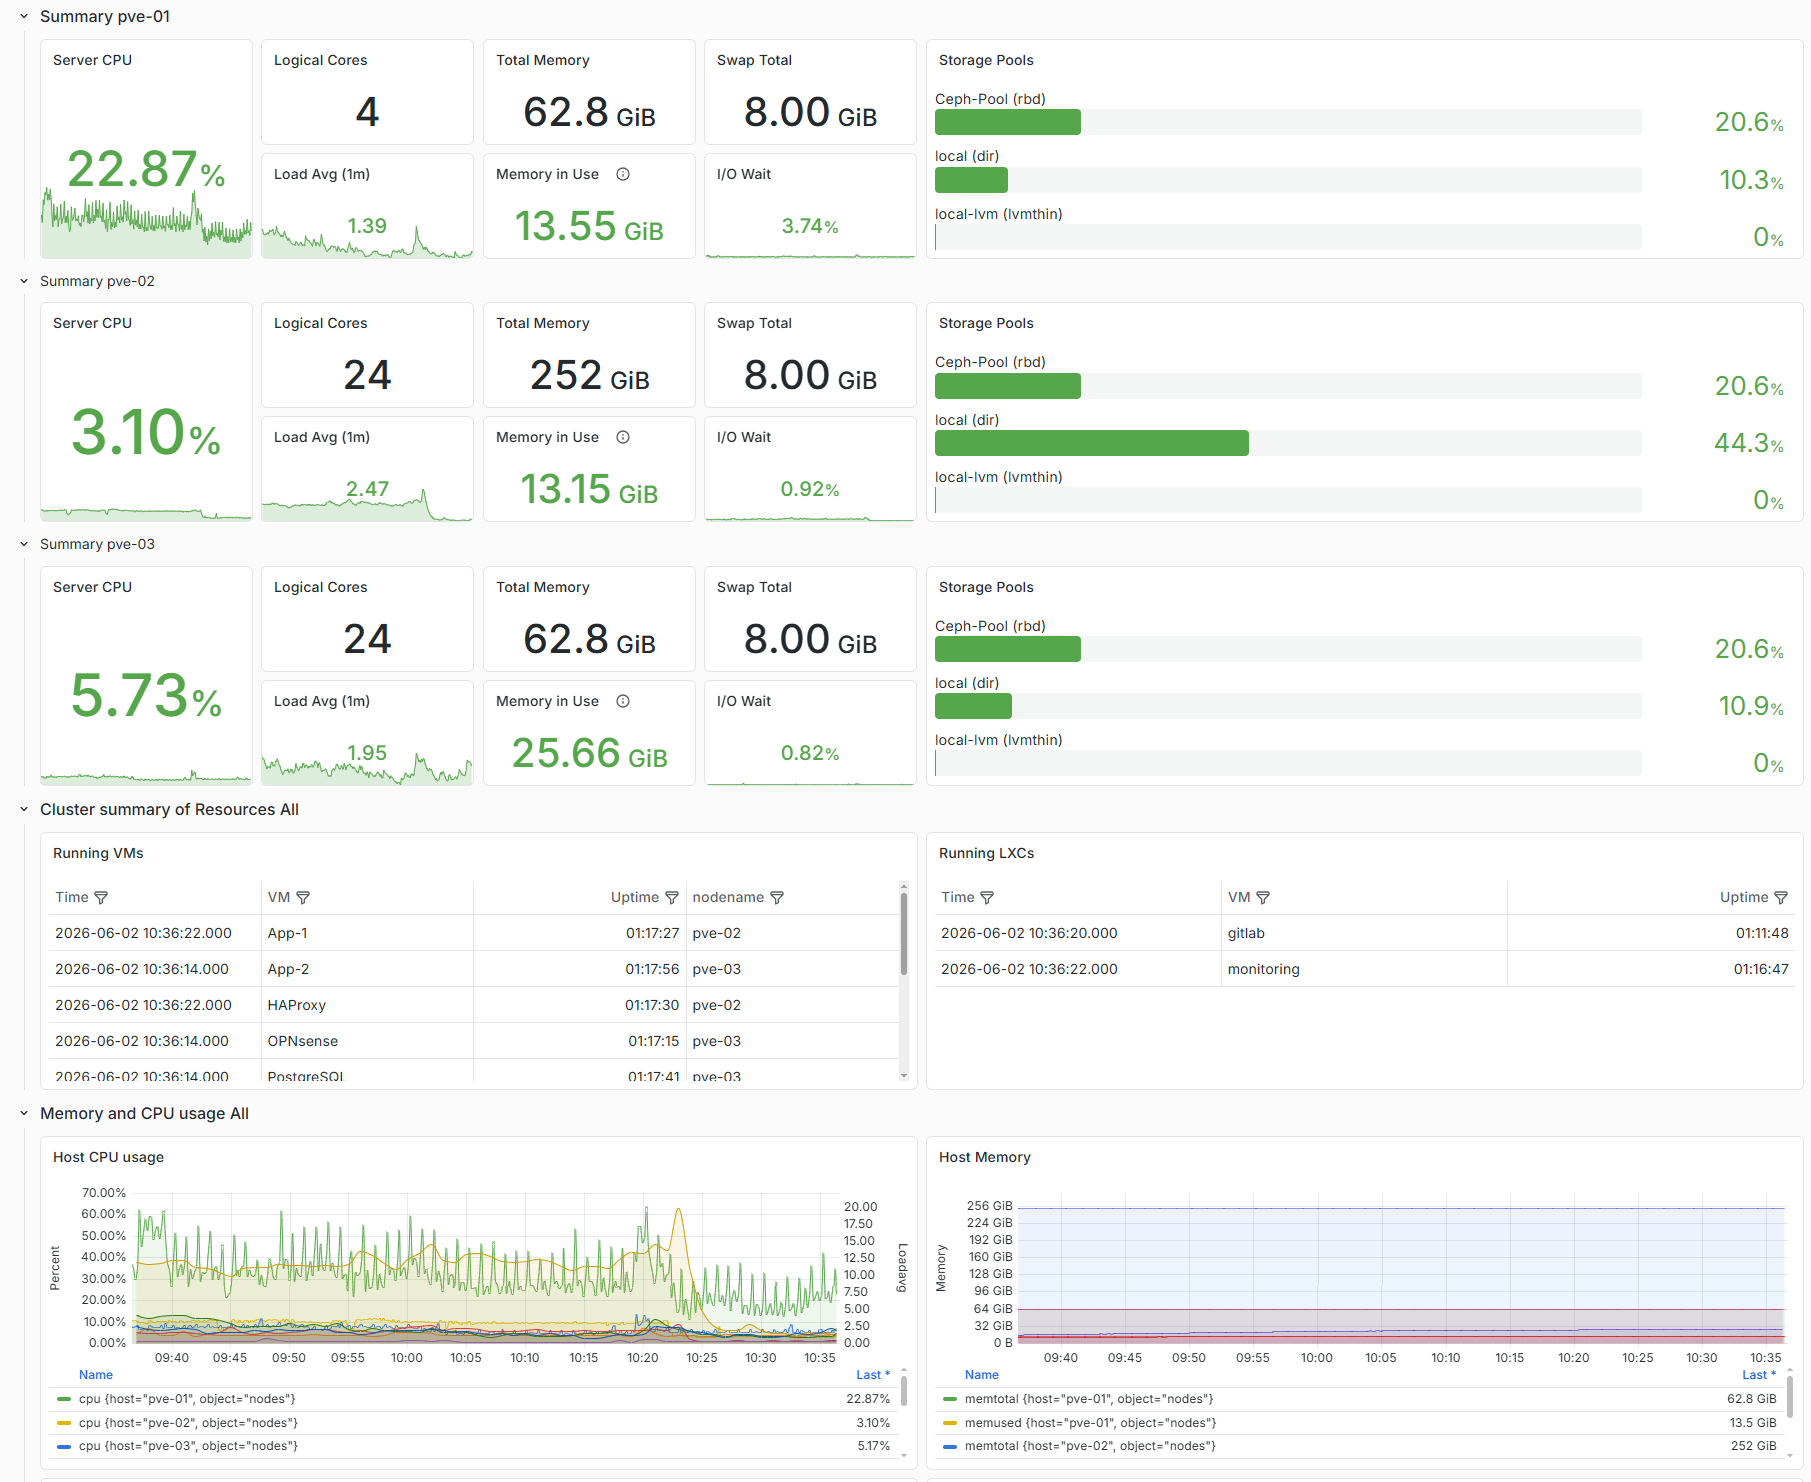
\includegraphics[width=1\textwidth]{image/ch4/grafana cluster dashboard_full.png}
    \caption{Dashboard Grafana Infrastructure -- vue complète des métriques CPU, mémoire et réseau des trois nœuds Proxmox.}
    \label{fig:ann-grafana-proxmox-full}
\end{figure}

\par Ce tableau de bord, alimenté par InfluxDB via le mécanisme natif ``Metric Server'' de Proxmox, affiche en temps réel l'utilisation du CPU, la mémoire disponible, la charge réseau et le nombre de VMs en cours d'exécution pour chacun des trois nœuds PVE-01, PVE-02 et PVE-03. Les séries temporelles permettent d'identifier les tendances de charge sur les dernières heures et de corréler les événements de migration CLBS avec l'évolution des ressources.\\

\section*{A.2 \quad Dashboard Cluster Ceph}

\begin{figure}[H]
    \centering
    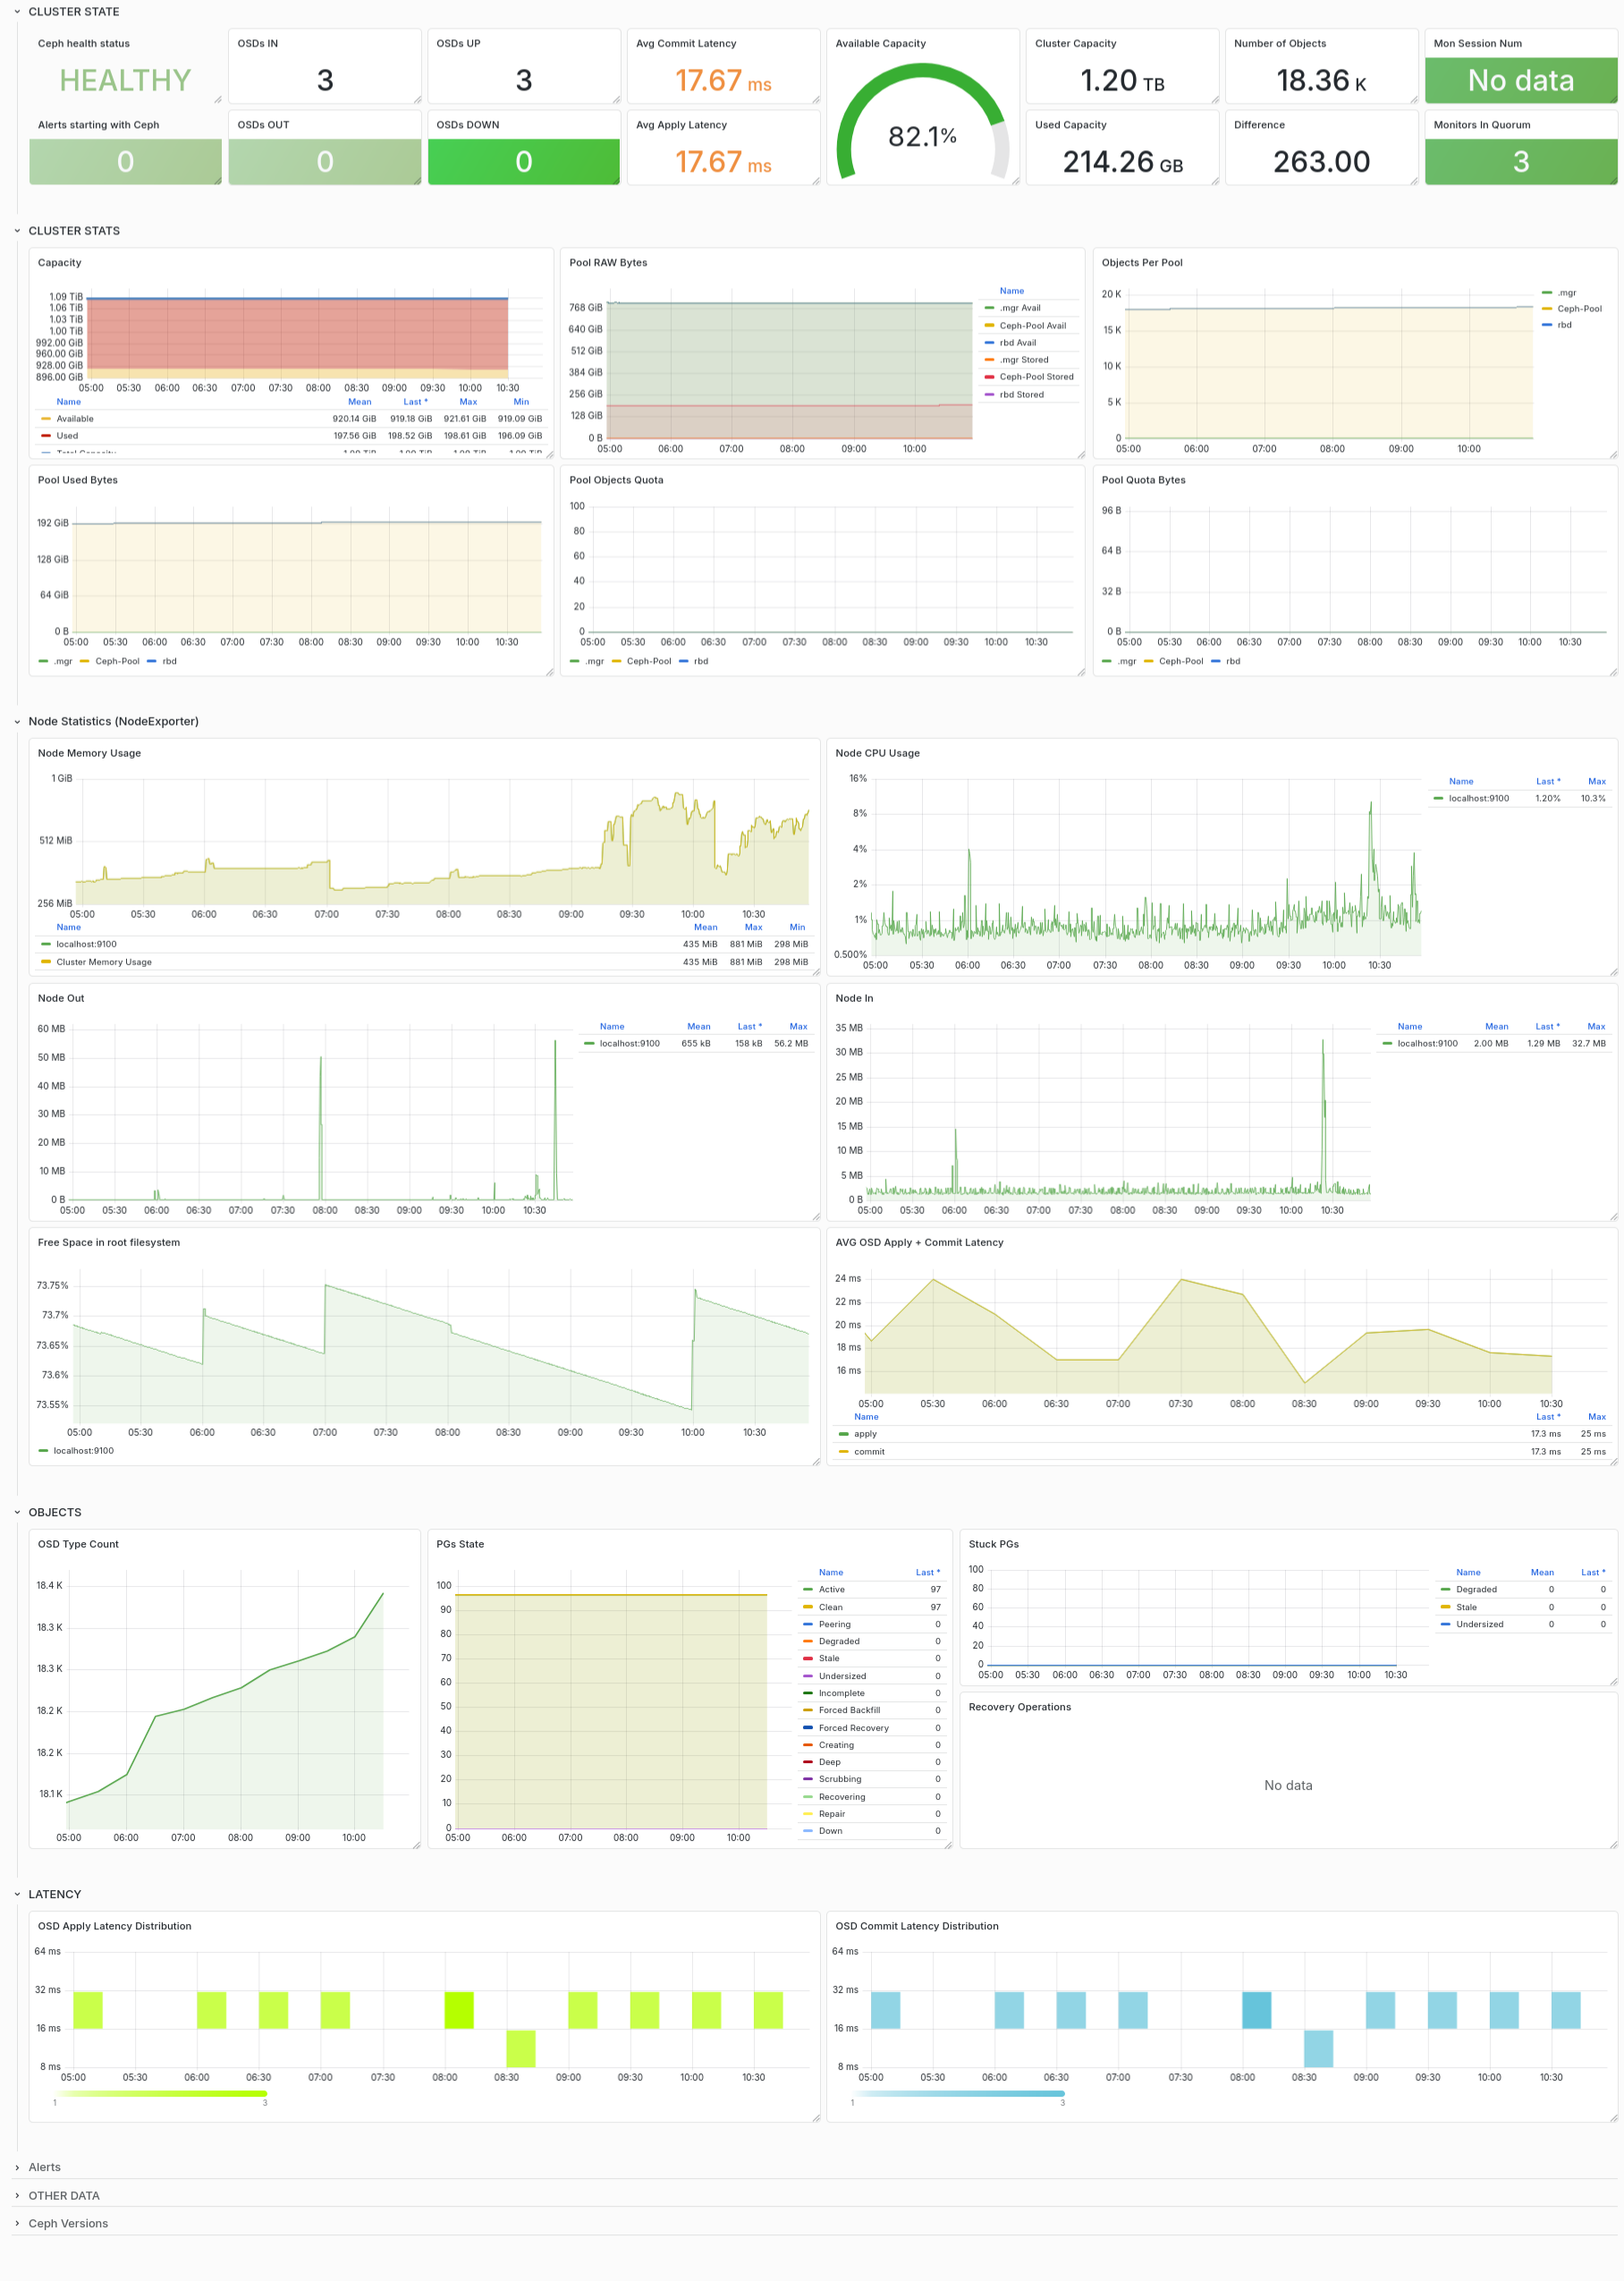
\includegraphics[width=1\textwidth]{image/ch4/grafana_ceph_dashboard_full.png}
    \caption{Dashboard Grafana Ceph -- vue complète de l'état du cluster, des pools et de la latence des OSDs.}
    \label{fig:ann-grafana-ceph-full}
\end{figure}

\par Ce tableau de bord, alimenté par Prometheus via le module MGR Ceph, centralise les métriques de santé du cluster : état global (\texttt{HEALTH\_OK}/\texttt{HEALTH\_WARN}), capacité utilisée et disponible par pool, débit I/O en lecture et écriture, latence des OSDs et taux de réplication en temps réel. Il constitue la vue de référence pour diagnostiquer tout incident affectant la couche stockage.\\

\section*{A.3 \quad Journaux Système via Loki}

\begin{figure}[H]
    \centering
    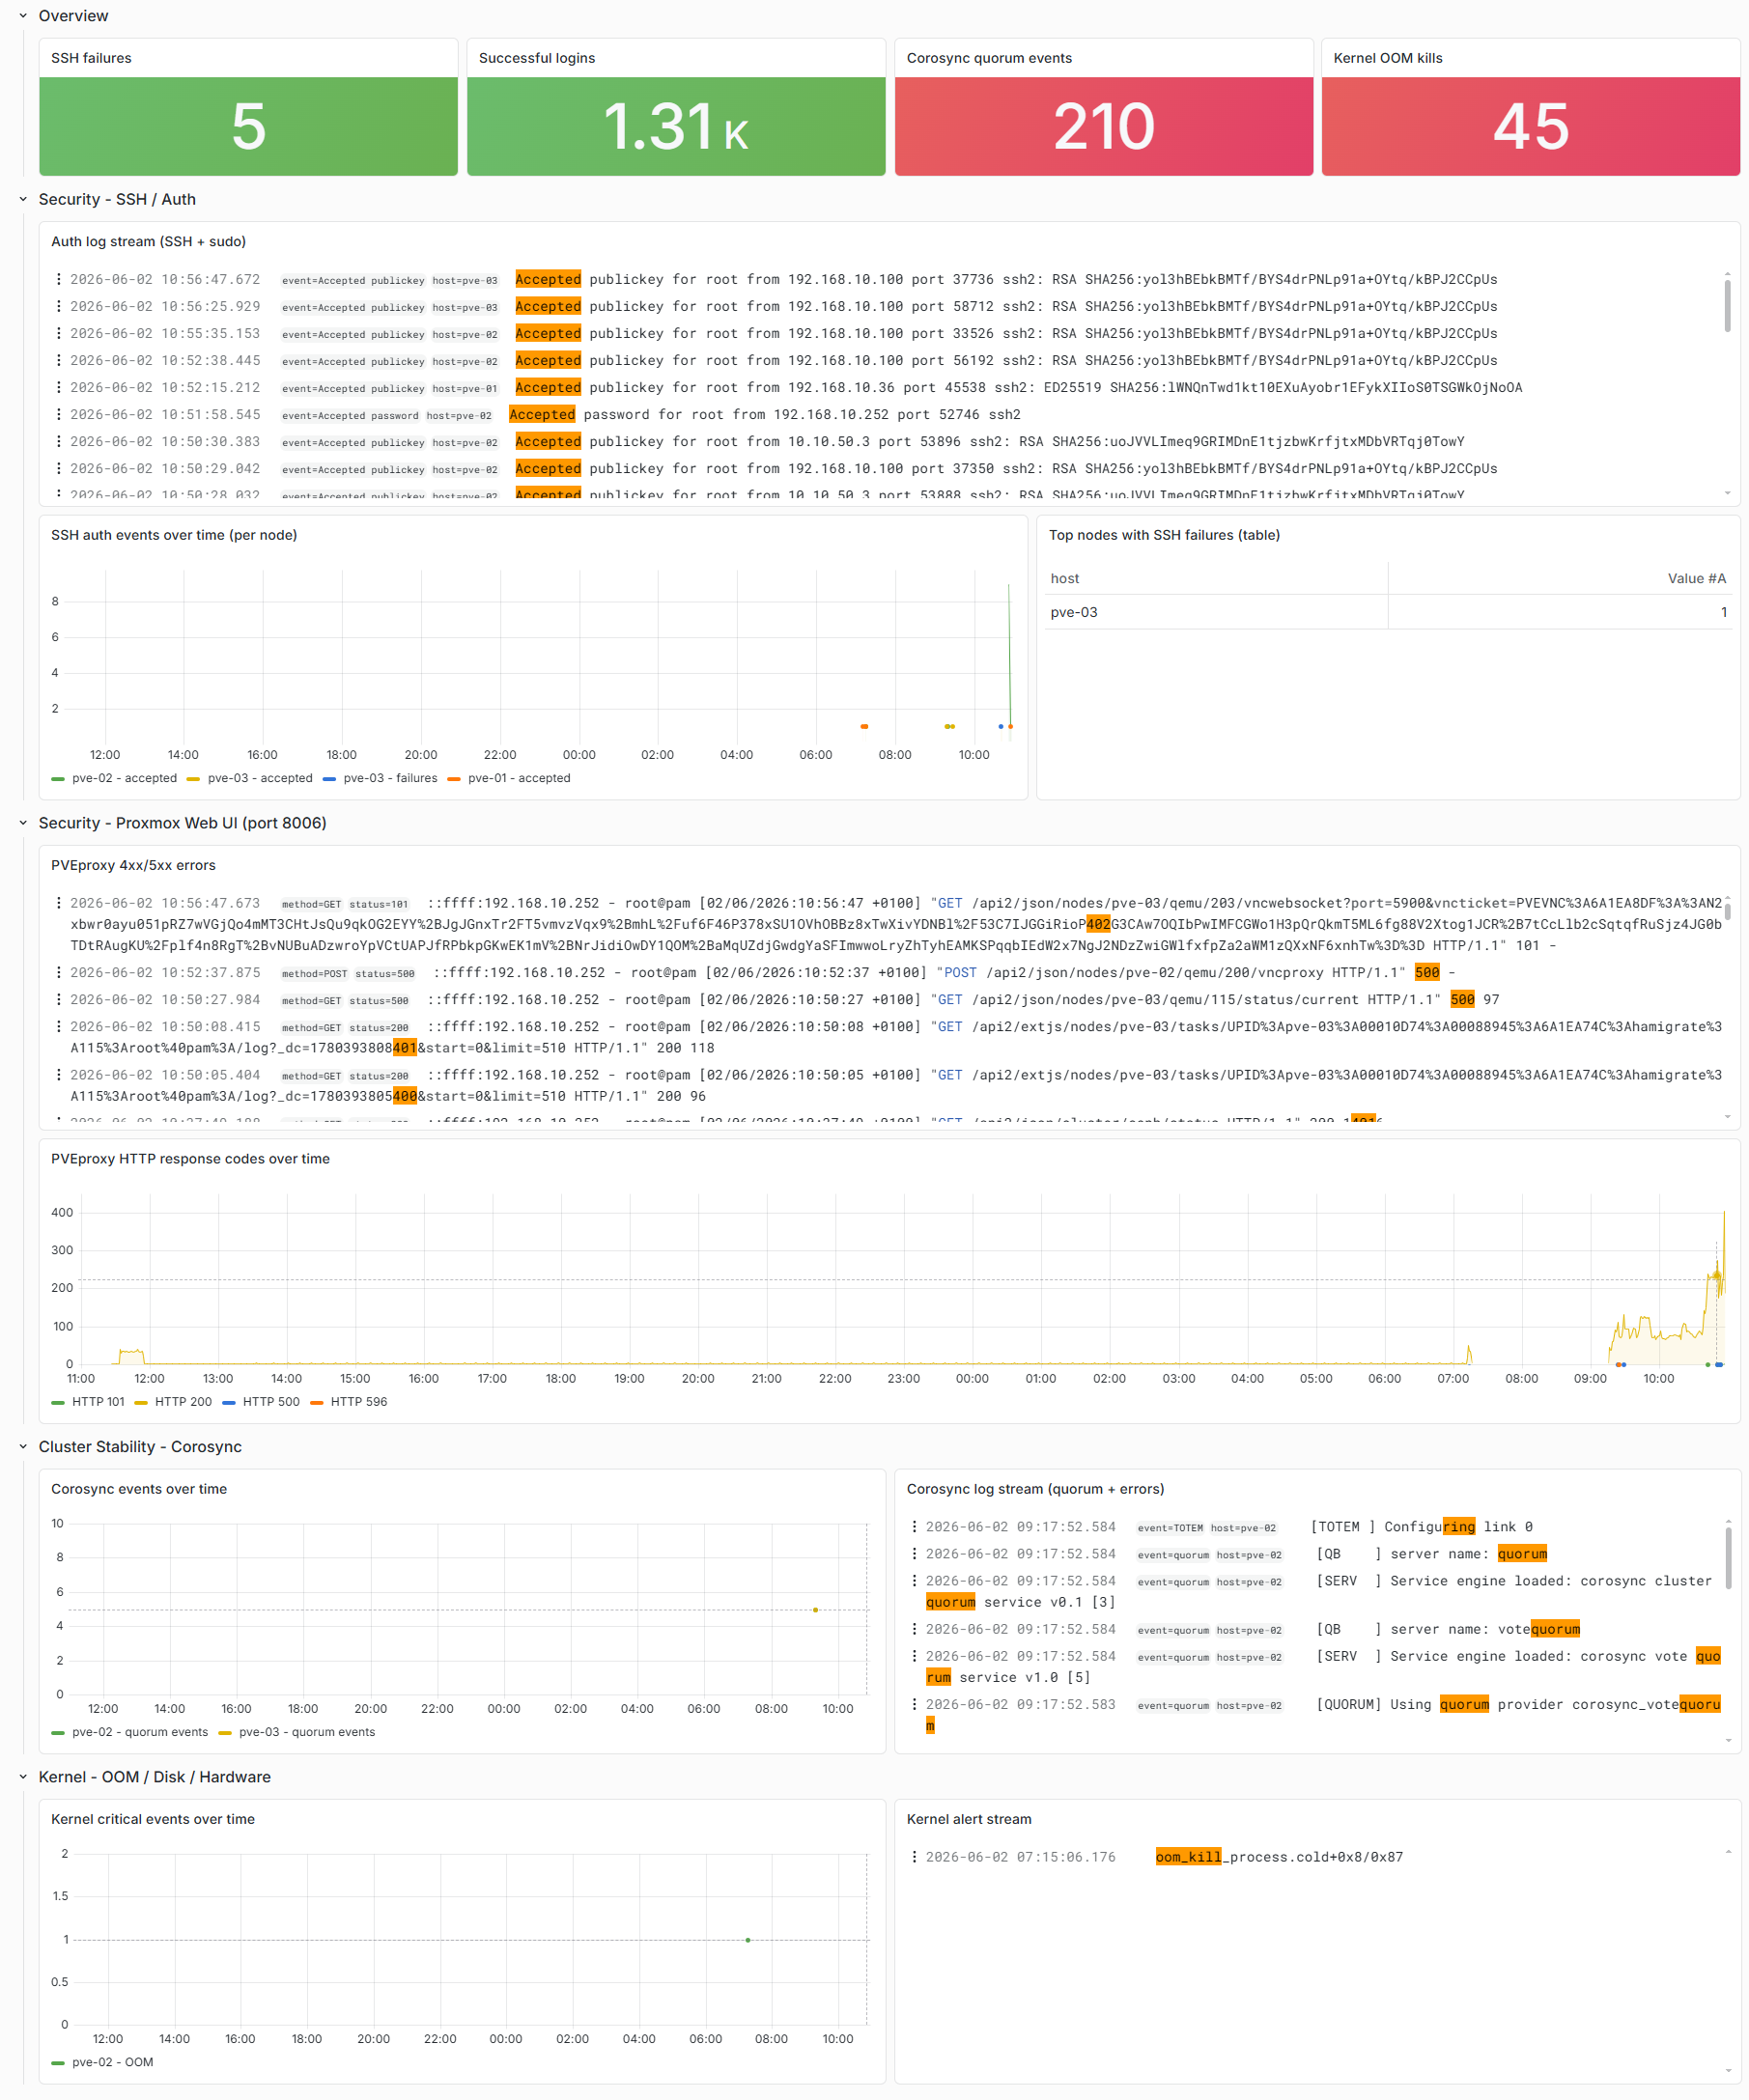
\includegraphics[width=1\textwidth]{image/ch4/grafana syslog dashboard_full.png}
    \caption{Dashboard Grafana Loki -- journaux système centralisés des nœuds Proxmox et des VMs.}
    \label{fig:ann-grafana-loki-full}
\end{figure}

\par Ce tableau de bord, utilisant Loki comme source de données dans Grafana, permet d'interroger les journaux système de l'ensemble des nœuds et VMs via le langage LogQL. Les logs sont filtrables par hôte (label \texttt{host}), par fichier source (label \texttt{filename}) et par niveau de sévérité. Cette vue unifiée coexiste avec les tableaux de bord de métriques, offrant une corrélation directe entre les événements système et les variations de charge.\\

% ============================================================
\chapter{Configuration Complète des Interfaces Réseau}
\label{ann:vxlan}
% ============================================================

\par Cette annexe présente le fichier \texttt{/etc/network/interfaces} complet de chacun des trois nœuds Proxmox. Ces fichiers définissent l'ensemble des tunnels VxLAN point-à-point en maillage complet ainsi que les bridges OVS associés. Seule l'adresse IP du bridge de management et les adresses des interfaces internes diffèrent d'un nœud à l'autre.\\

\section*{B.1 \quad Configuration complète de PVE-01}

\begin{lstlisting}[style=sonacode,language={},caption={Fichier /etc/network/interfaces complet -- PVE-01 (192.168.10.100)},label={lst:ann-pve01-full}]
auto lo
iface lo inet loopback

iface nic0 inet manual

auto vmbr0
iface vmbr0 inet static
    address 192.168.10.100/24
    gateway 192.168.10.36
    ovs_type OVSBridge
    ovs_ports nic0

auto nic0
iface nic0 inet manual
    ovs_type OVSPort
    ovs_bridge vmbr0

iface nic1 inet manual
iface nic2 inet manual
iface nic3 inet manual

# ===== COROSYNC VXLAN (key=20) =====
auto vxlan20-pve02
iface vxlan20-pve02 inet manual
    ovs_type OVSPort
    ovs_bridge vmbr0
    ovs_options type=vxlan options:remote_ip=192.168.10.213 options:key=20

auto vxlan20-pve03
iface vxlan20-pve03 inet manual
    ovs_type OVSPort
    ovs_bridge vmbr0
    ovs_options type=vxlan options:remote_ip=192.168.10.84 options:key=20

auto vxlan20-int
iface vxlan20-int inet static
    address 10.10.20.1/24
    ovs_type OVSIntPort
    ovs_bridge vmbr0

# ===== CEPH INTERNE VXLAN (key=30) =====
auto vxlan30-pve02
iface vxlan30-pve02 inet manual
    ovs_type OVSPort
    ovs_bridge vmbr0
    ovs_options type=vxlan options:remote_ip=192.168.10.213 options:key=30

auto vxlan30-pve03
iface vxlan30-pve03 inet manual
    ovs_type OVSPort
    ovs_bridge vmbr0
    ovs_options type=vxlan options:remote_ip=192.168.10.84 options:key=30

auto vxlan30-int
iface vxlan30-int inet static
    address 10.10.30.1/24
    ovs_type OVSIntPort
    ovs_bridge vmbr0

# ===== CEPH PUBLIC VXLAN (key=40) =====
auto vxlan40-pve02
iface vxlan40-pve02 inet manual
    ovs_type OVSPort
    ovs_bridge vmbr0
    ovs_options type=vxlan options:remote_ip=192.168.10.213 options:key=40

auto vxlan40-pve03
iface vxlan40-pve03 inet manual
    ovs_type OVSPort
    ovs_bridge vmbr0
    ovs_options type=vxlan options:remote_ip=192.168.10.84 options:key=40

auto vxlan40-int
iface vxlan40-int inet static
    address 10.10.40.1/24
    ovs_type OVSIntPort
    ovs_bridge vmbr0

# ===== MIGRATION LIVE VXLAN (key=50) =====
auto vxlan50-pve02
iface vxlan50-pve02 inet manual
    ovs_type OVSPort
    ovs_bridge vmbr0
    ovs_options type=vxlan options:remote_ip=192.168.10.213 options:key=50

auto vxlan50-pve03
iface vxlan50-pve03 inet manual
    ovs_type OVSPort
    ovs_bridge vmbr0
    ovs_options type=vxlan options:remote_ip=192.168.10.84 options:key=50

auto vxlan50-int
iface vxlan50-int inet static
    address 10.10.50.1/24
    ovs_type OVSIntPort
    ovs_bridge vmbr0

# ===== SAUVEGARDE VXLAN (key=90) =====
auto vxlan90-pve02
iface vxlan90-pve02 inet manual
    ovs_type OVSPort
    ovs_bridge vmbr0
    ovs_options type=vxlan options:remote_ip=192.168.10.213 options:key=90

auto vxlan90-pve03
iface vxlan90-pve03 inet manual
    ovs_type OVSPort
    ovs_bridge vmbr0
    ovs_options type=vxlan options:remote_ip=192.168.10.84 options:key=90

auto vxlan90-int
iface vxlan90-int inet static
    address 10.10.90.1/24
    ovs_type OVSIntPort
    ovs_bridge vmbr0

# ===== VXLAN 60 (Dev) =====
auto vxlan60-pve02
iface vxlan60-pve02 inet manual
    ovs_type OVSPort
    ovs_bridge vmbr0
    ovs_options type=vxlan options:remote_ip=192.168.10.213 options:key=60

auto vxlan60-pve03
iface vxlan60-pve03 inet manual
    ovs_type OVSPort
    ovs_bridge vmbr0
    ovs_options type=vxlan options:remote_ip=192.168.10.84 options:key=60

auto vxlan60-int
iface vxlan60-int inet static
    ovs_type OVSIntPort
    ovs_bridge vmbr0

# ===== VXLAN 70 (Prod) =====
auto vxlan70-pve02
iface vxlan70-pve02 inet manual
    ovs_type OVSPort
    ovs_bridge vmbr0
    ovs_options type=vxlan options:remote_ip=192.168.10.213 options:key=70

auto vxlan70-pve03
iface vxlan70-pve03 inet manual
    ovs_type OVSPort
    ovs_bridge vmbr0
    ovs_options type=vxlan options:remote_ip=192.168.10.84 options:key=70

auto vxlan70-int
iface vxlan70-int inet static
    ovs_type OVSIntPort
    ovs_bridge vmbr0

# ===== VXLAN 80 (DMZ) =====
auto vxlan80-pve02
iface vxlan80-pve02 inet manual
    ovs_type OVSPort
    ovs_bridge vmbr0
    ovs_options type=vxlan options:remote_ip=192.168.10.213 options:key=80

auto vxlan80-pve03
iface vxlan80-pve03 inet manual
    ovs_type OVSPort
    ovs_bridge vmbr0
    ovs_options type=vxlan options:remote_ip=192.168.10.84 options:key=80

auto vxlan80-int
iface vxlan80-int inet static
    ovs_type OVSIntPort
    ovs_bridge vmbr0

# ===== VM Bridges =====
auto vmbr60
iface vmbr60 inet manual
    bridge_ports vxlan60-int
    bridge_stp off
    bridge_fd 0

auto vmbr70
iface vmbr70 inet manual
    bridge_ports vxlan70-int
    bridge_stp off
    bridge_fd 0

auto vmbr80
iface vmbr80 inet manual
    bridge_ports vxlan80-int
    bridge_stp off
    bridge_fd 0

source /etc/network/interfaces.d/*
\end{lstlisting}

\section*{B.2 \quad Configuration complète de PVE-02}

\begin{lstlisting}[style=sonacode,language={},caption={Fichier /etc/network/interfaces complet -- PVE-02 (192.168.10.213)},label={lst:ann-pve02-full}]
auto lo
iface lo inet loopback

iface nic0 inet manual

auto vmbr0
iface vmbr0 inet static
    address 192.168.10.213/24
    gateway 192.168.10.36
    ovs_type OVSBridge
    ovs_ports nic0

auto nic0
iface nic0 inet manual
    ovs_type OVSPort
    ovs_bridge vmbr0

iface nic1 inet manual
iface nic2 inet manual
iface nic3 inet manual

# ===== COROSYNC VXLAN (key=20) =====
auto vxlan20-pve01
iface vxlan20-pve01 inet manual
    ovs_type OVSPort
    ovs_bridge vmbr0
    ovs_options type=vxlan options:remote_ip=192.168.10.100 options:key=20

auto vxlan20-pve03
iface vxlan20-pve03 inet manual
    ovs_type OVSPort
    ovs_bridge vmbr0
    ovs_options type=vxlan options:remote_ip=192.168.10.84 options:key=20

auto vxlan20-int
iface vxlan20-int inet static
    address 10.10.20.2/24
    ovs_type OVSIntPort
    ovs_bridge vmbr0

# ===== CEPH INTERNE VXLAN (key=30) =====
auto vxlan30-pve01
iface vxlan30-pve01 inet manual
    ovs_type OVSPort
    ovs_bridge vmbr0
    ovs_options type=vxlan options:remote_ip=192.168.10.100 options:key=30

auto vxlan30-pve03
iface vxlan30-pve03 inet manual
    ovs_type OVSPort
    ovs_bridge vmbr0
    ovs_options type=vxlan options:remote_ip=192.168.10.84 options:key=30

auto vxlan30-int
iface vxlan30-int inet static
    address 10.10.30.2/24
    ovs_type OVSIntPort
    ovs_bridge vmbr0

# ===== CEPH PUBLIC VXLAN (key=40) =====
auto vxlan40-pve01
iface vxlan40-pve01 inet manual
    ovs_type OVSPort
    ovs_bridge vmbr0
    ovs_options type=vxlan options:remote_ip=192.168.10.100 options:key=40

auto vxlan40-pve03
iface vxlan40-pve03 inet manual
    ovs_type OVSPort
    ovs_bridge vmbr0
    ovs_options type=vxlan options:remote_ip=192.168.10.84 options:key=40

auto vxlan40-int
iface vxlan40-int inet static
    address 10.10.40.2/24
    ovs_type OVSIntPort
    ovs_bridge vmbr0

# ===== MIGRATION LIVE VXLAN (key=50) =====
auto vxlan50-pve01
iface vxlan50-pve01 inet manual
    ovs_type OVSPort
    ovs_bridge vmbr0
    ovs_options type=vxlan options:remote_ip=192.168.10.100 options:key=50

auto vxlan50-pve03
iface vxlan50-pve03 inet manual
    ovs_type OVSPort
    ovs_bridge vmbr0
    ovs_options type=vxlan options:remote_ip=192.168.10.84 options:key=50

auto vxlan50-int
iface vxlan50-int inet static
    address 10.10.50.2/24
    ovs_type OVSIntPort
    ovs_bridge vmbr0

# ===== SAUVEGARDE VXLAN (key=90) =====
auto vxlan90-pve01
iface vxlan90-pve01 inet manual
    ovs_type OVSPort
    ovs_bridge vmbr0
    ovs_options type=vxlan options:remote_ip=192.168.10.100 options:key=90

auto vxlan90-pve03
iface vxlan90-pve03 inet manual
    ovs_type OVSPort
    ovs_bridge vmbr0
    ovs_options type=vxlan options:remote_ip=192.168.10.84 options:key=90

auto vxlan90-int
iface vxlan90-int inet static
    address 10.10.90.2/24
    ovs_type OVSIntPort
    ovs_bridge vmbr0

# ===== VXLAN 60 (Dev) =====
auto vxlan60-pve01
iface vxlan60-pve01 inet manual
    ovs_type OVSPort
    ovs_bridge vmbr0
    ovs_options type=vxlan options:remote_ip=192.168.10.100 options:key=60

auto vxlan60-pve03
iface vxlan60-pve03 inet manual
    ovs_type OVSPort
    ovs_bridge vmbr0
    ovs_options type=vxlan options:remote_ip=192.168.10.84 options:key=60

auto vxlan60-int
iface vxlan60-int inet static
    ovs_type OVSIntPort
    ovs_bridge vmbr0

# ===== VXLAN 70 (Prod) =====
auto vxlan70-pve01
iface vxlan70-pve01 inet manual
    ovs_type OVSPort
    ovs_bridge vmbr0
    ovs_options type=vxlan options:remote_ip=192.168.10.100 options:key=70

auto vxlan70-pve03
iface vxlan70-pve03 inet manual
    ovs_type OVSPort
    ovs_bridge vmbr0
    ovs_options type=vxlan options:remote_ip=192.168.10.84 options:key=70

auto vxlan70-int
iface vxlan70-int inet static
    ovs_type OVSIntPort
    ovs_bridge vmbr0

# ===== VXLAN 80 (DMZ) =====
auto vxlan80-pve01
iface vxlan80-pve01 inet manual
    ovs_type OVSPort
    ovs_bridge vmbr0
    ovs_options type=vxlan options:remote_ip=192.168.10.100 options:key=80

auto vxlan80-pve03
iface vxlan80-pve03 inet manual
    ovs_type OVSPort
    ovs_bridge vmbr0
    ovs_options type=vxlan options:remote_ip=192.168.10.84 options:key=80

auto vxlan80-int
iface vxlan80-int inet static
    ovs_type OVSIntPort
    ovs_bridge vmbr0

# ===== VM Bridges =====
auto vmbr60
iface vmbr60 inet manual
    bridge_ports vxlan60-int
    bridge_stp off
    bridge_fd 0

auto vmbr70
iface vmbr70 inet manual
    bridge_ports vxlan70-int
    bridge_stp off
    bridge_fd 0

auto vmbr80
iface vmbr80 inet manual
    bridge_ports vxlan80-int
    bridge_stp off
    bridge_fd 0

source /etc/network/interfaces.d/*
\end{lstlisting}

\section*{B.3 \quad Configuration complète de PVE-03}

\begin{lstlisting}[style=sonacode,language={},caption={Fichier /etc/network/interfaces complet -- PVE-03 (192.168.10.84)},label={lst:ann-pve03-full}]
auto lo
iface lo inet loopback

iface nic0 inet manual

auto vmbr0
iface vmbr0 inet static
    address 192.168.10.84/24
    gateway 192.168.10.36
    ovs_type OVSBridge
    ovs_ports nic0

auto nic0
iface nic0 inet manual
    ovs_type OVSPort
    ovs_bridge vmbr0

iface nic1 inet manual
iface nic2 inet manual
iface nic3 inet manual

# ===== COROSYNC VXLAN (key=20) =====
auto vxlan20-pve01
iface vxlan20-pve01 inet manual
    ovs_type OVSPort
    ovs_bridge vmbr0
    ovs_options type=vxlan options:remote_ip=192.168.10.100 options:key=20

auto vxlan20-pve02
iface vxlan20-pve02 inet manual
    ovs_type OVSPort
    ovs_bridge vmbr0
    ovs_options type=vxlan options:remote_ip=192.168.10.213 options:key=20

auto vxlan20-int
iface vxlan20-int inet static
    address 10.10.20.3/24
    ovs_type OVSIntPort
    ovs_bridge vmbr0

# ===== CEPH INTERNE VXLAN (key=30) =====
auto vxlan30-pve01
iface vxlan30-pve01 inet manual
    ovs_type OVSPort
    ovs_bridge vmbr0
    ovs_options type=vxlan options:remote_ip=192.168.10.100 options:key=30

auto vxlan30-pve02
iface vxlan30-pve02 inet manual
    ovs_type OVSPort
    ovs_bridge vmbr0
    ovs_options type=vxlan options:remote_ip=192.168.10.213 options:key=30

auto vxlan30-int
iface vxlan30-int inet static
    address 10.10.30.3/24
    ovs_type OVSIntPort
    ovs_bridge vmbr0

# ===== CEPH PUBLIC VXLAN (key=40) =====
auto vxlan40-pve01
iface vxlan40-pve01 inet manual
    ovs_type OVSPort
    ovs_bridge vmbr0
    ovs_options type=vxlan options:remote_ip=192.168.10.100 options:key=40

auto vxlan40-pve02
iface vxlan40-pve02 inet manual
    ovs_type OVSPort
    ovs_bridge vmbr0
    ovs_options type=vxlan options:remote_ip=192.168.10.213 options:key=40

auto vxlan40-int
iface vxlan40-int inet static
    address 10.10.40.3/24
    ovs_type OVSIntPort
    ovs_bridge vmbr0

# ===== MIGRATION LIVE VXLAN (key=50) =====
auto vxlan50-pve01
iface vxlan50-pve01 inet manual
    ovs_type OVSPort
    ovs_bridge vmbr0
    ovs_options type=vxlan options:remote_ip=192.168.10.100 options:key=50

auto vxlan50-pve02
iface vxlan50-pve02 inet manual
    ovs_type OVSPort
    ovs_bridge vmbr0
    ovs_options type=vxlan options:remote_ip=192.168.10.213 options:key=50

auto vxlan50-int
iface vxlan50-int inet static
    address 10.10.50.3/24
    ovs_type OVSIntPort
    ovs_bridge vmbr0

# ===== SAUVEGARDE VXLAN (key=90) =====
auto vxlan90-pve01
iface vxlan90-pve01 inet manual
    ovs_type OVSPort
    ovs_bridge vmbr0
    ovs_options type=vxlan options:remote_ip=192.168.10.100 options:key=90

auto vxlan90-pve02
iface vxlan90-pve02 inet manual
    ovs_type OVSPort
    ovs_bridge vmbr0
    ovs_options type=vxlan options:remote_ip=192.168.10.213 options:key=90

auto vxlan90-int
iface vxlan90-int inet static
    address 10.10.90.3/24
    ovs_type OVSIntPort
    ovs_bridge vmbr0

# ===== VXLAN 60 (Dev) =====
auto vxlan60-pve01
iface vxlan60-pve01 inet manual
    ovs_type OVSPort
    ovs_bridge vmbr0
    ovs_options type=vxlan options:remote_ip=192.168.10.100 options:key=60

auto vxlan60-pve02
iface vxlan60-pve02 inet manual
    ovs_type OVSPort
    ovs_bridge vmbr0
    ovs_options type=vxlan options:remote_ip=192.168.10.213 options:key=60

auto vxlan60-int
iface vxlan60-int inet static
    ovs_type OVSIntPort
    ovs_bridge vmbr0

# ===== VXLAN 70 (Prod) =====
auto vxlan70-pve01
iface vxlan70-pve01 inet manual
    ovs_type OVSPort
    ovs_bridge vmbr0
    ovs_options type=vxlan options:remote_ip=192.168.10.100 options:key=70

auto vxlan70-pve02
iface vxlan70-pve02 inet manual
    ovs_type OVSPort
    ovs_bridge vmbr0
    ovs_options type=vxlan options:remote_ip=192.168.10.213 options:key=70

auto vxlan70-int
iface vxlan70-int inet static
    ovs_type OVSIntPort
    ovs_bridge vmbr0

# ===== VXLAN 80 (DMZ) =====
auto vxlan80-pve01
iface vxlan80-pve01 inet manual
    ovs_type OVSPort
    ovs_bridge vmbr0
    ovs_options type=vxlan options:remote_ip=192.168.10.100 options:key=80

auto vxlan80-pve02
iface vxlan80-pve02 inet manual
    ovs_type OVSPort
    ovs_bridge vmbr0
    ovs_options type=vxlan options:remote_ip=192.168.10.213 options:key=80

auto vxlan80-int
iface vxlan80-int inet static
    ovs_type OVSIntPort
    ovs_bridge vmbr0

# ===== VM Bridges =====
auto vmbr60
iface vmbr60 inet manual
    bridge_ports vxlan60-int
    bridge_stp off
    bridge_fd 0

auto vmbr70
iface vmbr70 inet manual
    bridge_ports vxlan70-int
    bridge_stp off
    bridge_fd 0

auto vmbr80
iface vmbr80 inet manual
    bridge_ports vxlan80-int
    bridge_stp off
    bridge_fd 0

source /etc/network/interfaces.d/*
\end{lstlisting}

% ============================================================
\chapter{Résultat d'Exécution Rundeck}
\label{ann:rundeck}
% ============================================================

\par Cette annexe présente le résultat d'une exécution complète d'un job Rundeck déclenché depuis l'interface web. Le job exécuté est \textbf{Provision VM}, qui invoque le playbook Ansible \texttt{provision\_vm.yml} pour créer une machine virtuelle à partir du template Debian stocké dans le pool Ceph.\\

\begin{figure}[H]
  \centering
  \fbox{\parbox{0.85\textwidth}{\textit{[CAPTURE À INSÉRER]}}}
  \caption{Résultat d'exécution d'un job Rundeck avec le journal Ansible complet.}
  [CAPTURE : dans Rundeck $\to$ Activity, ouvrir le détail d'une exécution
  récente, capturer la page affichant le statut \texttt{Succeeded} et les
  tâches Ansible déroulées avec leurs états (ok, changed, skipped)]
  \label{fig:rundeck-execution}
\end{figure}

\par La Figure~\ref{fig:rundeck-execution} présente la page de détail d'une exécution Rundeck. On y observe le statut global \texttt{Succeeded}, le nom du job déclenché, la durée d'exécution et le journal Ansible complet listant chaque tâche avec son état (\texttt{ok}, \texttt{changed} ou \texttt{skipped}). Le bouton ``Re-run'' permet de relancer le même job avec les mêmes paramètres sans repasser par le formulaire de création.\\
